\documentclass[../../doc.tex]{subfiles}
\graphicspath{{\subfix{../../img}}}
\begin{document}
    \subsection{Алгоритм}
    С учетом вышесказанного можно построить следующий алгоритм.
    Алгоритмы \ref{alg:BackwardPass}, \ref{alg:ForwardPass} демонстрируют обратный и прямой проход для получения оптимальной поправки.
    Алгоритм \ref{alg:Sinthesis} демонстрирует общий алгоритм построения управления.

    Продемонстрируем работу алгоритма для классической задачи перехода в целевое состояние~$x^{\textnormal{final}}$ без фазовых ограничений.
    Для этого будем использовать следующие компоненты функции цены:
    \begin{equation}\label{eq:ilqr-algo:cost}
        q^{\textnormal{final}}(x) = \left\|x - x^{\textnormal{final}}\right\|^2,
        \qquad
        q(x) \equiv 0.
    \end{equation}
    Начальным референсным управлением выберем
    \begin{equation}\label{eq:ilqr-algo:ref-control}
        \bar u^k = 0,\; k = \overline{1, N}.
    \end{equation}
    \clearpage
    \RestyleAlgo{ruled}
    \begin{rusalgorithm}\caption{Обратный проход}\label{alg:BackwardPass}
        \DontPrintSemicolon
        \SetKwProg{Function}{function}{\;begin}{end function}
        \Function{BackwardPass($\bar u$, $\bar x$)}{
            $S_{N+1}, v^{N+1} \gets $ \eqref{eq:method-s-v-boundary-result}\;
            \For{$k \gets N$ \KwTo $1$}{
                $S_k, v^{k} \gets $ \eqref{eq:method-s-v-result}\;
            }
            \Return{S, v}
        }
    \end{rusalgorithm}
    \RestyleAlgo{ruled}
    \begin{rusalgorithm}\caption{Прямой проход}\label{alg:ForwardPass}
        \DontPrintSemicolon
        \SetKwProg{Function}{function}{\;begin}{end function}
        \SetKwRepeat{Do}{do}{while}
        \Function{ForwardPass($\bar u$, $\bar x$, $J_{\textnormal{prev}}$)}{
            $\eta \gets 1$\;
            \Do{$\frac{J_{\textnormal{prev}} - J}{J_{\delta}(0) - J_{\delta}(\delta u)} \notin [\xi_1, \xi_2]$}{
                $\delta x^0 \gets 0$\;
                \For{$k \gets 1$ \KwTo $N$}{
                    $\delta u^k, \delta x^{k+1} \gets$ \eqref{eq:method-optimal-control-result}, \eqref{eq:ref-system} \;
                    $u^k \gets \bar u^k + \delta u^k$\;
                }
                $J \gets$ \eqref{eq:discrete-cost} \;
                $\eta \gets \gamma \eta$\;
            }
            \Return{u, J}
        }
    \end{rusalgorithm}
    
    \RestyleAlgo{ruled}
    \begin{rusalgorithm}\caption{Синтез управления}\label{alg:Sinthesis}
        \DontPrintSemicolon
        \SetKwProg{Function}{function}{\;begin}{end function}
        \SetKwRepeat{Do}{do}{while}
        \Function{Synthesis($\bar u$)}{
            $J \gets $ \eqref{eq:discrete-cost}\;
            \Do{$|J - J_{\textnormal{prev}}| \geqslant \varepsilon$}{
                $J_{\textnormal{prev}} \gets J$\;
                $\bar x \gets$ \eqref{eq:discrete-system}\;
                $S, v \gets \textnormal{BackwardPass}(\bar u, \bar x)$\;
                $u, J \gets \textnormal{ForwardPass}(S, v, J_{\textnormal{prev}})$\;
            }
            \Return{u}
        }
    \end{rusalgorithm}

    \begin{figure}[h]
        \begin{center}
            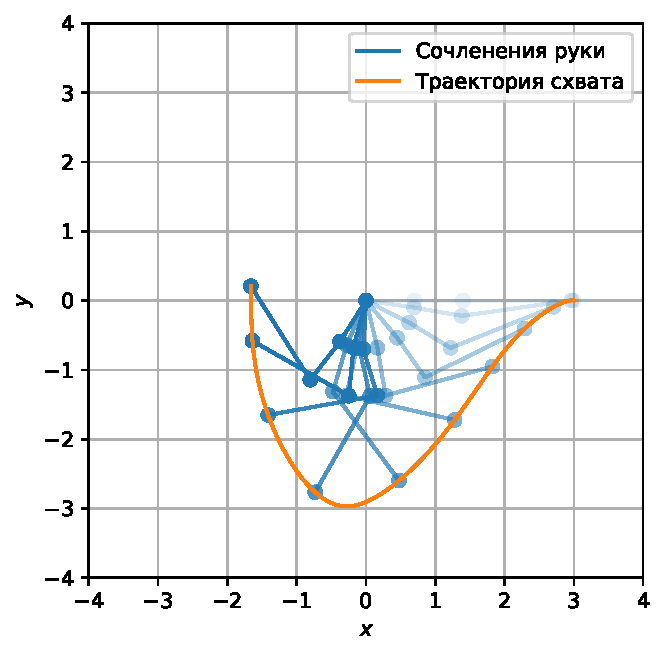
\includegraphics[width=0.49\textwidth]{iLQR/pendulum}
            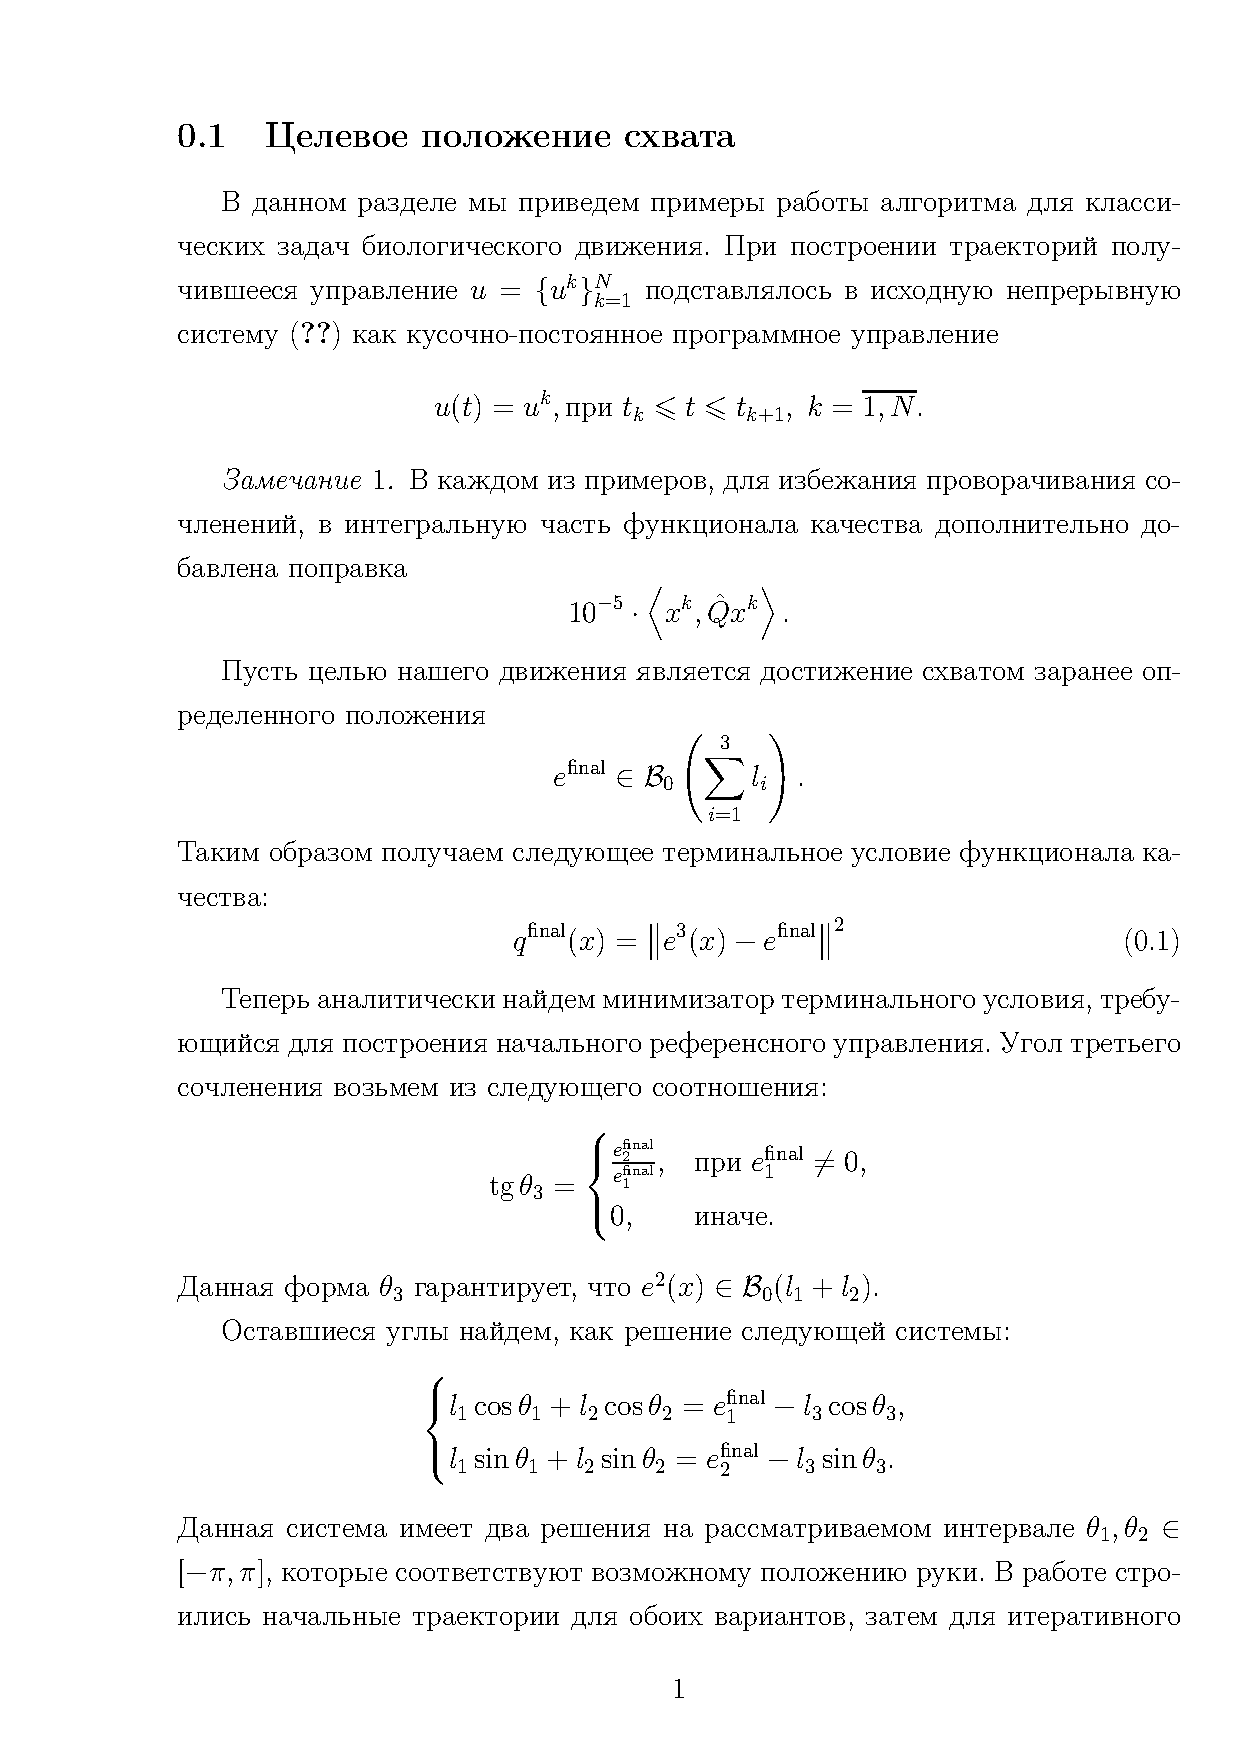
\includegraphics[width=0.49\textwidth]{iLQR/endpoint}
        \end{center}
        \caption{
            Решение задачи перехода в целевое состояние \eqref{eq:ilqr-algo:cost} c начальным референсным управлением \eqref{eq:ilqr-algo:ref-control}.
            Слева: поведение системы при полученном управлении. Справа: траектории схвата на каждой итерации алгоритма, более ранние итерации показаны бледнее.
            Алгоритм сошелся на $14$ итерации.
        }
    \end{figure}

    \ifSubfilesClassLoaded{
        \nocite{*}
        \clearpage
        \bibliographystyle{plain}
        \bibliography{../../refs}
    }{}
\end{document}